\section{Exercises}
\label{ANOVAExercises}

\begin{problem}
%Un epidemiólogo desea comparar tres variantes de una vacuna para la brucelosis bovina. Se seleccionaron 75 animales que posteriormente fueron repartidos al azar en los tres grupos que posteriormente recibieron cada una de las variantes. Las respuestas de los anticuerpos se registraron dos semanas después para cada animal. A continuación se muestran algunos resultados obtenidos junto con algunas preguntas que debes resolver:
  A epidemiologist wants to compare three types of vaccine against
  brucellosis in cattle. With that purpose 103 cows were randomized in
  three groups for each of the type of vaccines. The response of the
  antibodies was measured two weeks later for every individual. 
\begin{enumerate}
\item This graphic shows the values got for each animal. Do you
  think that ANOVA test will detect any difference according to the
  figure? Do you think that they will meet the conditions to apply
  ANOVA? 
  % A continuación se muestra una representación gráfica de los resultados obtenidos. ¿Qué crees que se obtendrá como resultado de un análisis de la varianza? ¿Crees que se cumplirán las hipótesis de aplicabilidad?
\begin{center}
  \includegraphics[width=7cm]{./ch_07a_inference_for_means_oi_biostat/figures/eoce/tema7-5}
  \%label{Fig1}
\end{center}

\item We got the following outcome with the computer:
    \begin{itemize}
    \item Levene's test (p-value=0.3758)
    \item Type 1:  Shapiro-Wilk Test (p-value=0.4567)
    \item Type 2:  Shapiro-Wilk Test(p-value=0.4538)
    \item Type  3: Shapiro-Wilk Test (p-value=0.0834)
    \end{itemize}
    Set a hypothesis testing and explain your
    conclusion for each p-value. Are fulfilled  the conditions for
    ANOVA? 
   % Plantea el contraste correspondiente a cada p-valor y explica las conclusiones que se deriva de cada uno de ellos.
    %¿Se cumplen todas las hipótesis de aplicabilidad del ANOVA? Justifica tu respuesta

\item The ANOVA  test statistic is $F=35.3$
    \begin{parts}
    \item  What distribution is used to calculate the acceptance interval% ¿En qué distribución nos fijaremos para calcular la región de rechazo?
    \item Calculate the acceptance interval with a significance level $\alpha=0.05$
    \item Is ANOVA test enough to know which pairs of treatments are
      going to be different %A partir del ANOVA podemos saber qué tratamientos difieren entre sí y cuáles no?
    \end{parts}

\item The computer displays the following graph and data for a pairwise
  comparison: 



\begin{tabular}{|c|c|c|c|}
  \hline
  % after \\: \hline or \cline{col1-col2} \cline{col3-col4} ...
   & Diference& 95\% interval& 95\% Interval\\
  Comparison& Sample mean & Lower Limit& Upper Limit \\

  \hline
  2-1 & 1.03 & 0.53 & 1.54 \\
  3-1 & 1.56 & 1.05 & 2.06 \\
  3-2 & 0.42 & 0.02 & 1.02 \\
  \hline
\end{tabular}

\begin{center}
  \includegraphics[width=7cm]{./ch_07a_inference_for_means_oi_biostat/figures/eoce/tema7-6}
\end{center}

\end{enumerate}

\end{problem}

\begin{problem}
%\eoce{ \qt{Bladder cancer}
%Se desea valorar si existen diferencias significativas en el tiempo medio de recuperación de una intervención quirúrgica,
%para la extirpación de un tumor en la vejiga en perros, según tres técnicas quirúrgicas: A (Laparoscopia),
%B (Cirugía abierta clásica), C (Cirugía abierta innovadora).
%Para llevar a cabo el estudio se tomó una muestra de 58 pacientes con este tipo de tumor y
%se les aplicó, al azar, una de las tres técnicas. 25 pacientes fueron intervenidos por laparoscopia,
%13 pacientes fueron intervenidos por cirugía abierta clásica y 20 por innovadora.
%Según los resultados que aparecen a continuación,\\
  A medical department wants to determine whether there exists significant difference in
  the recovering time of a surgery to remove a  tumor in the
  urinary bladder using three techniques: A (laparoscopy), B
  (conventional surgery) and  C (minimally invasive procedure) .
  They selected 58 patients with this kind of tumor and they were
  randomized to one of techniques: 25 patients underwent  laparoscopy,
  13 conventional procedure and 20 were operated with the minimally
  invasive procedure.

  The conditions of ANOVA were checked with the following tests: \\
  Levene's test (p-value= 0.6082)\\
Procedure A: Shapiro - Wilk Test (p-value= 0.3444)\\
Procedure B: Shapiro - Wilk Test (p-value= 0.5688)\\
Procedure C: Shapiro - Wilk Test (p-value= 0.3060)\\
ANOVA: F=80.13\\

\begin{tabular}{|c|c|c|c|}
  \hline
  % after \\: \hline or \cline{col1-col2} \cline{col3-col4} ...
   & Difference &  95\%  Interval&  95\% Interval\\
  Comparison & Sample mean & Lower Lim & Upper Lim   \\  \hline
  B-A & 8.43 & 6.06 & 10.80 \\
  C-A & 10.28 & 8.20 & 12.36 \\
  C-B & 1.85 & -0.61 & 4.32 \\
  \hline
\end{tabular}

$ $\\
\begin{parts}
\item Are all the conditions met to apply ANOVA?
 \item Set hypothesis testing of ANOVA and write your conclusions
   according to the data provided in the text.
   \item What are your conclusions according to Tuckey's pairwise
     comparison test?
\end{parts}
%a) ¿Se cumplen los criterios de aplicabilidad del ANOVA? Justifica tu respuesta, escribiendo los contrastes necesarios para la discusión.

%b) Escribe el contraste al que contesta la prueba ANOVA y razona a qué conclusión conduce su resultado.

%c) A partir de la prueba ANOVA, ¿podemos saber qué técnicas quirúrgicas difieren entre si? Justifica la respuesta.

%rd) Comenta las conclusiones que se deducen de las comparaciones de Tukey.


% }{}
\end{problem}
% 37


% 38
\begin{problem}
 % \eoce{\qt{Student performance across discussion sections}
    A professor who teaches a large introductory statistics class (197 students) with eight discussion sections would like to test if student performance differs by discussion section, where each discussion section has a different teaching assistant. The summary table below shows the average final exam score for each discussion section as well as the standard deviation of scores and the number of students in each section.
\begin{center}
\begin{tabular}{rrrrrrrrr}
  \hline
 			& Sec 1 & Sec 2 & Sec 3 & Sec 4 & Sec 5 & Sec 6 & Sec 7 & Sec 8 \\ 
  \hline
$n_i$		& 33 & 19 & 10 & 29 & 33 & 10 & 32 & 31 \\ 
$\bar{x}_i$	& 92.94 & 91.11 & 91.80 & 92.45 & 89.30 & 88.30 & 90.12 & 93.35 \\ 
$s_i$ 		& 4.21 & 5.58 & 3.43 & 5.92 & 9.32 & 7.27 & 6.93 & 4.57 \\ 
   \hline
\end{tabular}
\end{center}
The ANOVA output below can be used to test for differences between the average scores from the different discussion sections.
\begin{center}
\begin{tabular}{lrrrrr}
\hline
 			& Df 		& Sum Sq & Mean Sq 	& F value & Pr($>$F) \\ 
\hline
section 		& 7 		& 525.01 	& 75.00 		& 1.87 	& 0.0767 \\ 
Residuals 	& 189	& 7584.11	& 40.13 		&  		&  \\ 
\hline
\end{tabular}
\end{center}
Conduct a hypothesis test to determine if these data provide convincing evidence that the average score varies across some (or all) groups. Check conditions and describe any assumptions you must make to proceed with the test.
%}{}
\end{problem}
% 39 


% 41
\begin{problem}
% \eoce{\qt{GPA and major}
Undergraduate students taking an introductory statistics course at Duke University conducted a survey about GPA and major. The side-by-side box plots show the distribution of GPA among three groups of majors. Also provided is the ANOVA output.

\begin{center}
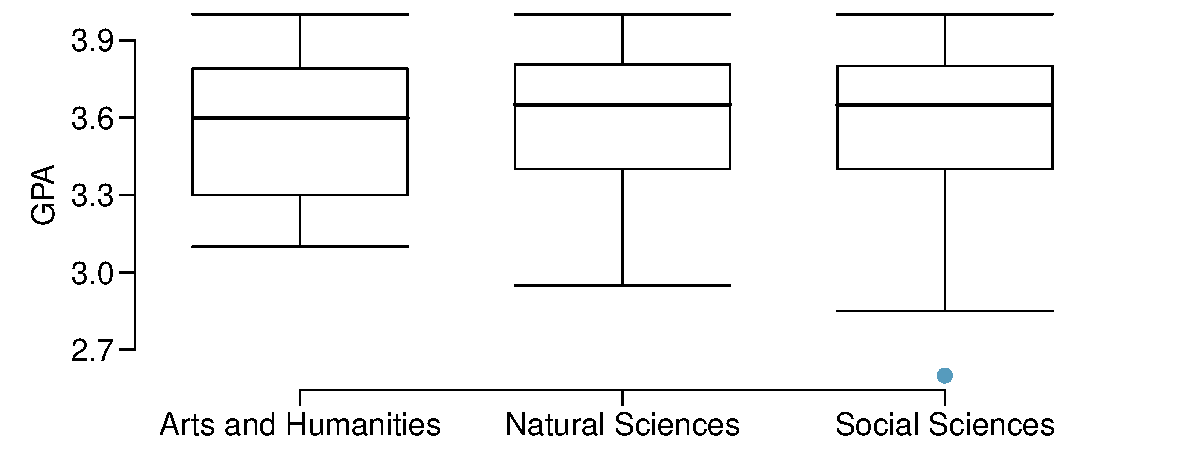
\includegraphics[width=0.8\textwidth]{./ch_07a_inference_for_means_oi_biostat/figures/eoce/gpa_major/gpa_major}
\end{center}
\begin{center}
\begin{tabular}{lrrrrr}
  \hline
 & Df & Sum Sq & Mean Sq & F value & Pr($>$F) \\ 
  \hline
major & 2 & 0.03 & 0.02 & 0.21 & 0.8068 \\ 
  Residuals & 195 & 15.77 & 0.08 &  &  \\ 
   \hline
\end{tabular}
\end{center}
\begin{parts}
\item Write the hypotheses for testing for a difference between average GPA across majors.
\item What is the conclusion of the hypothesis test?
\item How many students answered these questions on the survey, i.e. what is the sample size?
\end{parts}
% }{}
\end{problem}


